\documentclass[10pt, a4paper]{extarticle}
\usepackage[utf8]{inputenc}
\usepackage[left=1.9cm,right=1.9cm,top=1.9cm,bottom=1.9cm]{geometry}
\usepackage[T1]{fontenc}
\usepackage{amssymb}
\usepackage{tgpagella}
\usepackage{graphicx}
\usepackage{fancyhdr}
\usepackage{amsmath}
\usepackage{answers}
\usepackage{lastpage}
\usepackage{enumerate}
\usepackage{array}
\usepackage{tikz}
\usepackage{tikz-3dplot}
\usepackage{array,multirow,makecell}
\usepackage{mdwlist}
\usepackage{systeme}
\usepackage{relsize} 
\usepackage{siunitx}
\usepackage{multirow}
\usepackage{lscape}
\usepackage{makecell}
\usepackage{xcolor}
\usepackage{setspace}
\usepackage{lipsum} 
\usepackage{url}
\usepackage{hyperref}
\usepackage{breakurl}
\usepackage[french]{babel} 
\usepackage{multicol}
\usepackage{eurosym}
\usepackage{chngcntr}

\newcolumntype{M}[1]{>{\raggedright}m{#1}}

\definecolor{onered}{RGB}{198,200,234}
\onehalfspacing

\numberwithin{equation}{section}
\newcommand*{\rttensor}[1]{\bar{\bar{#1}}}
\numberwithin{figure}{section}

\begin{document}

\fancyhf{}
\renewcommand{\headrulewidth}{.6pt}
 
\fancyhead[R]{\large \bf T\'el\'ecom Paris\\   
Ann\'ee universitaire : 2024/2025\\ }
\fancyhead[L]{
\includegraphics[width=5cm]{TP.png}}
\pagestyle{fancy}

\vspace*{40mm}
\begin{center}
    \Huge
    
    \textbf{CSC\_4IM01\_TP : Introduction au Traitement des Images}\vspace*{1mm}\\
\begin{tikzpicture}
\draw[very thin] (-13,0) -- (1,0);
\end{tikzpicture}
\vspace*{26mm}\\
\Huge
\fboxsep0.6em
\textbf{Restauration d'Images Sous-marines}
\vspace*{11mm}\\
\end{center}
\vspace*{50mm}
\begin{center}
\textbf{\Large Fouad KHELIFI}\vspace{2mm}\\ 
\textbf{\Large Hortense BONNEAU} 
\end{center}
\vspace*{25mm}
\textbf{Encadrant : Yann GOUSSEAU} 
\newpage
\fancyhf{}
\renewcommand{\headrulewidth}{.6pt}
\fancyhead[L]{\textbf{CSC\_4IM01\_TP}}
\fancyhead[R]{\small \leftmark}
\setlength{\headheight}{10pt}
\renewcommand{\footrulewidth}{.6pt}
\fancyfoot[C]{\thepage}
\pagestyle{fancy}
\tableofcontents
\newpage

\section{\'Etat de l'Art du Traitement des Images Sous-Marines}
\counterwithin{figure}{section}
\subsection{Introduction}
\par Le traitement des images sous-marines est crucial pour surmonter les limitations inhérentes à l'environnement aquatique, comme la faible visibilité, le flou, et la dominante bleue causée par l'absorption et la diffusion de la lumière. Ces défis limitent la portée visuelle et la qualité des images, en particulier à de grandes profondeurs ou dans des eaux troubles. Les méthodes proposées pour résoudre ces problèmes se répartissent en deux catégories principales : \textbf{la restauration d'image} et \textbf{l'amélioration d'image}, chacune ayant des applications et des contraintes spécifiques.

\subsection{Méthodes de Restauration d'Image}
\par Les images sous-marines subissent une dégradation importante causée par l'absorption et la diffusion de la lumière. L'absorption réduit progressivement l'énergie lumineuse, supprimant les couleurs selon leur longueur d'onde (par exemple, le rouge disparaît après environ 3 mètres). La diffusion, quant à elle, provoque un flou et diminue le contraste, amplifiant le \textit{voile} visuel. Les techniques de restauration compensent ces effets par :
\begin{itemize}
\item[$\bullet$] \textbf{Modélisation physique :} Exploite les propriétés optiques de l'eau (absorption, diffusion) et des fonctions de transfert pour corriger flous et pertes de contraste.
\item[$\bullet$] \textbf{Déconvolution :} Applique des filtres, comme celui de Wiener, basés sur des fonctions mesurant la propagation lumineuse pour restaurer les détails.
\item[$\bullet$] \textbf{Analyse de polarisation :} Isolant la lumière diffusée grâce à des filtres polarisants, elle réduit les voiles optiques et améliore le contraste.
\end{itemize}
Ces méthodes, bien que précises, dépendent fortement des caractéristiques de l’environnement aquatique.

\subsection{Méthodes d'Amélioration d'Image}

\par Les techniques d’amélioration visent à optimiser la qualité visuelle des images sans nécessiter de modèles physiques complexes. Elles se concentrent sur la correction des couleurs, l'ajustement des contrastes et la suppression des dominantes chromatiques.
\begin{itemize}
\item[$\bullet$] \textbf{Espace $l\alpha\beta$ :} En convertissant les images dans un espace de couleur perceptuel, cette approche ajuste indépendamment la luminosité, la teinte et la saturation pour atténuer la dominante bleue et rehausser les détails visuels.
\item[$\bullet$] \textbf{Automatic Color Equalization (ACE) :} Inspirée de la perception humaine, cette méthode ajuste automatiquement les couleurs et le contraste pour compenser les dominantes dues à l’absorption sous-marine, offrant des images plus équilibrées et naturelles.
\end{itemize}
Le document met en avant et implémente spécifiquement ces deux méthodes, en raison de leur efficacité et de leur capacité à traiter rapidement des images sous-marines tout en améliorant leur rendu visuel. L'intégralité du code source ainsi que les images utilisées dans ce projet sont disponibles sur le dépôt GitHub accessible via \href{https://github.com/fouakh/Project-IMA201}{\colorbox{black}{\textcolor{white}{\textbf{ce lien.}}}}


\subsection{Méthodes par Apprentissage}
\par Il existe plusieurs méthodes par apprentissage qui se proposent de restaurer des images sous-marines, on peut citer par exemple :
\vspace{2mm}
\begin{itemize}
\item[$\bullet$] \textbf{Underwater Image Restoration via Contrastive Learning and a Real-World Dataset} : la restauration d’image sous-marines par
apprentissage contrastif tout en construisant une base de données d’images sur lesquelles s’appuyer pour entraîner l’algorithme. La méthode de transfert d’image à image non-supervisée repose sur de l’apprentissage contrastif en le combinant avec des réseaux antagonistes génératifs (GAN). Le but étant de maximiser l’information mutuelle entre patchs correspondants à l’image brute, et à l’image restaurée afin de pouvoir saisir les correspondances de contenu et les similarités de couleur entre les
deux domaines d’image.
\vspace{3mm}
\par Le concept de GAN est constitué de deux éléments : le générateur $G$ et le discriminateur $D$. Tandis que le générateur s’en tient à générer des images les plus réalistes possibles, le discriminateur lui, est chargé d’évaluer si les données générées sont réelles ou fausses. Comme les deux réseaux sont en compétition, cela permet d’améliorer progressivement la qualité des données générées.
\par La base de données d’image est divisée en trois parties : des images de basse qualité, des images de haute qualité et des images restaurées. Les images de bonne qualité sont associées à leur version
restaurée et constitue l’entrée et la référence d’un premier modèle supervisé, aussi appelé
\textit{apprentissage par paires}. Les images de plus basse qualité constituent l’entrée d’un second
modèle non-supervisé, cette fois avec comme référence d’images réelles, le set d’images restaurées.
Ce type d’apprentissage est dit \textit{sans paires}.
\vspace{2mm}
\par Afin d’effectuer le mappage, c’est-à-dire le processus de reconnaissance des correspondances d’un
ensemble de données à un autre, on extrait les caractéristiques des images identifiées depuis
différentes couches de l’encodeur du générateur que l’on redirige dans un Perceptron à deux
couches afin de pouvoir projeter ces caractéristiques dans un nouvel espace.
\vspace{2mm}
\par La méthode se propose de minimiser une fonction de perte générale, résultat de l’addition de trois
fonctions de pertes, pondérées par des paramètres.
\begin{itemize}
\item La première fonction de perte est celle de la perte antagoniste Adversarial Loss : elle permet de produire des images plus réalistiques.
\item La seconde fonction est celle de PatchNCE Loss : cette dernière vise à maximiser l’information mutuelle entre les patchs correspondants entre entrée et sortie du générateur.
\item Enfin la dernière est la fonction identité de perte, Identity Loss, qui encourage le générateur à éviter
tout changement de structure ou de couleur non-nécessaire entre l’entrée et la sortie.
\end{itemize}
\vspace{2mm}
Ensuite les deux modèles entraînés sont utilisés pour l’évaluation de l’algorithme.
\end{itemize}

\section{Correction des Couleurs à l'Aide de l'Espace RGB}

\subsection{Hypothèse du Monde Gris}
\par C'est l'hypothèse selon laquelle l'image devrait avoir, en moyenne, une couleur grise. C'est-à-dire que les moyennes des trois canaux de couleur (R, G, B) doivent être égales pour une scène correctement éclairée. Si ce n'est pas le cas, la correction de couleur va réajuster les valeurs de chaque canal pour compenser les biais de couleur.
\vspace{2mm}
\par L'idée de base de la correction est que, sous un éclairage uniforme, la somme des intensités des trois canaux (R, G, B) dans l'image devrait être équivalente, car la moyenne des couleurs d'une scène "idéale" sous lumière neutre devrait tendre vers le gris (même intensité dans les trois canaux).
\vspace{2mm}
\par Cette méthode est implémentée via la fonction \colorbox{gray!15}{\texttt{\textbf{process\_underwater\_image}}} qui est présente dans le fichier \colorbox{gray!15}{\texttt{\textbf{Undermarine\_lib.py}}}, de la manière suivante :

\begin{enumerate}
    \item \textbf{Calculer la moyenne de chaque canal (R, G, B) de l'image :}
    $$
    \bar{R} = \frac{1}{N} \sum_{x=1}^{N} R(x) \quad\quad\quad \bar{G} = \frac{1}{N} \sum_{x=1}^{N} G(x) \quad\quad\quad \bar{B} = \frac{1}{N} \sum_{x=1}^{N} B(x)
    $$
    où \( N \) est le nombre de pixels dans l'image, et \( R(x), G(x), B(x) \) sont les valeurs RGB du pixel \( x \).
    
    \item \textbf{Calculer la moyenne de l'illuminant} (moyenne des trois moyennes des canaux) :
    \[
    \bar{M} = \frac{\bar{R} + \bar{G} + \bar{B}}{3}
    \]

    \item \textbf{Ajuster les canaux pour égaliser les moyennes :} La correction consiste à ajuster les valeurs des canaux pour qu'ils aient tous la même moyenne. Pour chaque pixel, chaque composante de couleur (R, G, B) est divisée par sa moyenne respective et multipliée par la moyenne de l'illuminant :
    $$
    R_{\text{corr}}(x) = R(x) \times \frac{\bar{M}}{\bar{R}} \quad\quad\quad G_{\text{corr}}(x) = G(x) \times \frac{\bar{M}}{\bar{G}} \quad\quad\quad B_{\text{corr}}(x) = B(x) \times \frac{\bar{M}}{\bar{B}}
    $$
\end{enumerate}

\begin{figure}[h!]
\begin{center}
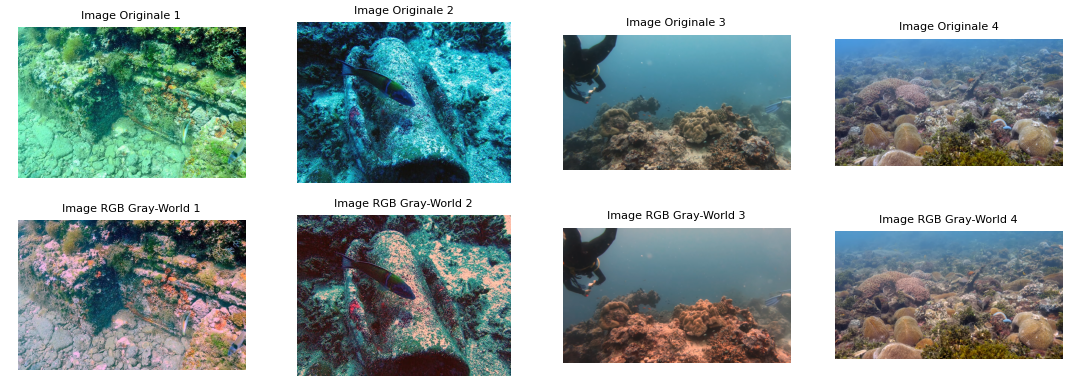
\includegraphics[width=18cm]{image004.png}
\end{center}
\label{figure2.1}
\caption{Résultats de la correction RGB (avec l'hypothèse du monde gris) sur des images sous-marines}
\end{figure} 

Comme illustré dans la \hyperref[figure2.1]{\textsc{Figure} 2.1} ( le reste des images traitées sont dans le fichier \colorbox{gray!15}{\texttt{\textbf{Images\_RGB\_GW}}}), pour les images ayant une composition variée et équilibrée, l'hypothèse du monde gris fonctionne correctement. Cependant, pour les images dominées par une couleur unique, comme celles contenant une grande étendue d'eau, la correction devient incorrecte. Sous l'eau, la lumière est principalement bleue, et l'algorithme, en cherchant à équilibrer les canaux, exagère la composante rouge. Cela résulte en une image où les objets hors de l'eau, comme les rochers ou les poissons, apparaissent avec une dominante rouge excessive, ce qui montre les limites de l'hypothèse du monde gris.

\subsection{Hypothèse des White Patches}\label{WP}

L’hypothèse des White Patches repose sur l’idée que certaines zones de l’image devraient être proches du blanc, même sous un éclairage non uniforme. En ajustant ces zones lumineuses (les "patchs blancs") pour qu'elles correspondent à un blanc idéal, on peut corriger les dominantes de couleur. Sur le principe on identifie les zones les plus lumineuses de l’image et on les ajuste pour qu’elles correspondent à un point blanc idéal \([255, 255, 255]\). Cela permet de corriger les dominantes de couleur sans affecter les autres zones de l’image.
\par Cette méthode est implémentée via la fonction \colorbox{gray!15}{\texttt{\textbf{process\_underwater\_image}}} qui est présente dans le fichier \colorbox{gray!15}{\texttt{\textbf{Undermarine\_lib.py}}}, de la manière suivante :

\begin{enumerate}
    \item \textbf{Conversion en niveaux de gris :} L'image est d'abord convertie en niveaux de gris pour identifier les zones les plus lumineuses noté $\text{Gray}(x)$
    
    \item \textbf{Identification des patchs lumineux :} On sélectionne les \( p\% \) des pixels les plus lumineux (par exemple, 2\% de l'image) comme étant les "patchs blancs" :
    \[
P_{\text{bright}} = \left\{ x \in \{1, \dots, N\} \mid \text{Gray}(x) \geq \theta \right\}
\]
Où :
\begin{itemize}
    \item[$\bullet$] \( P_{\text{bright}} \) représente l'ensemble des indices des pixels lumineux.
    \item[$\bullet$] \( \theta \) est un seuil qui détermine la luminosité maximale pour avoir $\#P_{\text{bright}} = \frac{p}{100} \times \#\text{Gray}$
\end{itemize}

    \item \textbf{Calcul de la moyenne des patchs lumineux :} La moyenne des couleurs des patchs lumineux est calculée :
    $$
    \bar{R}_{\text{bright}} = \frac{1}{\#P_{\text{bright}}} \sum_{x\in P_{\text{bright}}} R(x) \quad\quad\quad \bar{G}_{\text{bright}} = \frac{1}{\#P_{\text{bright}}} \sum_{x\in P_{\text{bright}}} G(x) \quad\quad\quad \bar{B}_{\text{bright}} = \frac{1}{\#P_{\text{bright}}} \sum_{x\in P_{\text{bright}}} B(x)
    $$

    \item \textbf{Application de la correction :} Un facteur de correction est appliqué à l'image pour ajuster les canaux \( R \), \( G \), et \( B \) qui est un réajustement du point blanc idéal.
    $$
    R_{\text{corr}}(x) = R(x) \times \frac{255}{\bar{R}_{\text{bright}}} \quad\quad\quad G_{\text{corr}}(x) = G(x) \times \frac{255}{\bar{G}_{\text{bright}}} \quad\quad\quad B_{\text{corr}}(x) = B(x) \times \frac{255}{\bar{B}_{\text{bright}}}
    $$
\end{enumerate}

\begin{figure}[h!]
\begin{center}
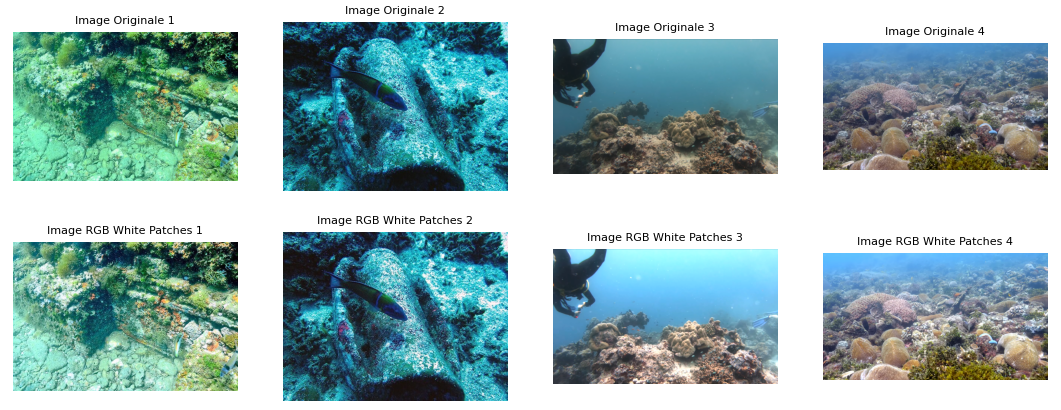
\includegraphics[width=18cm]{image005.png}
\end{center}
\label{figure2.2}
\caption{Résultats de la correction RGB (avec l'hypothèse des white patches avec $p=2\%$) }
\end{figure} 

\begin{figure}[h!]
\begin{center}
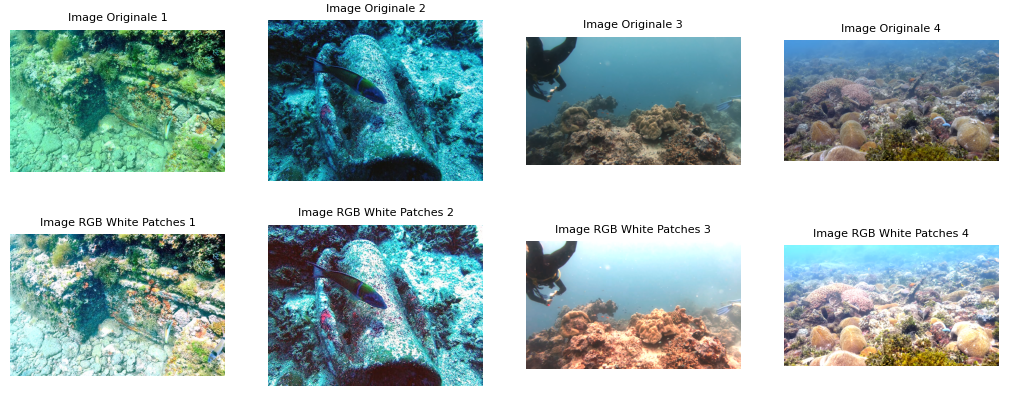
\includegraphics[width=18cm]{image010.png}
\end{center}
\label{figure2.3}
\caption{Résultats de la correction RGB (avec l'hypothèse des white patches avec $p=20\%$) }
\end{figure}

 \par Dans la \hyperref[figure2.2]{\textsc{Figure} 2.2} (le reste des images traitées sont dans le fichier \colorbox{gray!15}{\texttt{\textbf{Images\_RGB\_WP\_2p}}}), les deux premières images n'ont pas été corrigées, car l'hypothèse des patchs blancs n'est pas pertinente ici : bien qu'il y ait un \textit{voile} bleu, plusieurs zones blanches sont présentes, ce qui fausse l'application de cette méthode. Cependant, comme illustré dans la \hyperref[figure2.2]{\textsc{Figure} 2.3} (le reste des images traitées sont dans le fichier \colorbox{gray!15}{\texttt{\textbf{Images\_RGB\_WP\_20p}}}), en augmentant la valeur de \( p \), l'hypothèse des white patches devient progressivement valide même pour ces deux premières images, car un plus grand nombre de pixels lumineux est pris en compte, ce qui permet de capturer davantage de zones lumineuses pertinentes. Cette augmentation améliore la correction des dominantes colorées et permet d'obtenir des résultats proches de ceux de l'hypothèse du monde gris.
\vspace{3mm}
\par Cependant, augmenter excessivement la valeur de \( p \) peut engendrer des effets indésirables. En incluant trop de pixels dans la sélection des zones lumineuses, le facteur de correction devient biaisé par des zones qui ne devraient pas contribuer au calcul du point blanc. Cela peut entraîner une trop grande augmentation de la luminosité globale de l'image, rendant certaines zones surexposées et moins naturelles. Il est donc essentiel de choisir une valeur optimale de \( p \) qui équilibre la correction des couleurs et la préservation de la dynamique lumineuse de l'image.

\section{Correction des Couleurs à l'Aide de l'Espace $l\alpha\beta$}

\par Cette méthode repose sur une transformation dans l'espace colorimétrique perceptuel $l\alpha\beta$, qui un modèle de couleurs standardisé par la Commission Internationale de l'Éclairage (CIE) en 1976. Contrairement aux espaces colorimétriques comme RGB, qui sont basés sur des caractéristiques physiques de la lumière ou des pigments, l'espace $l\alpha\beta$ cherche à décrire les couleurs de manière plus uniforme et perceptuellement linéaire, ce qui signifie que les différences entre les couleurs dans cet espace correspondent mieux à ce que l'œil humain perçoit.

\subsection{Conversion dans l'Espace $l\alpha\beta$}

\par Les étapes de conversion décrites ci-dessous ont été implémentées dans la fonction \colorbox{gray!15}{\texttt{process\_underwater\_image}} du programme \colorbox{gray!15}{\texttt{\textbf{Undermarine\_lib.py}}}. On considère le vecteur \( F(x) = \left[ R(x), \;  G(x), \; B(x) \right]^T \), défini au pixel \( x \), où \( R(x) \), \( G(x) \), et \( B(x) \) sont les valeurs des trois canaux RGB normalisées dans l'intervalle \([0, 1]\).
\vspace{3mm}
\begin{enumerate}
    \item \textbf{Correction gamma :} Les valeurs RGB brutes issues du capteur ne représentent pas directement les intensités lumineuses physiques, car elles sont affectées par une courbe gamma non linéaire appliquée pour optimiser le rendu visuel. Alors une correction gamma inverse au gamma appliqué lors de la capture ou du rendu de l'image est appliquée:
\[
F'(x) = F(x)^{\frac{1}{\gamma}}
\]

    \item \textbf{Conversion RGB \(\to\) XYZ :}  
    Les valeurs RGB corrigées sont transformées dans l'espace XYZ, une représentation standard des couleurs perceptibles par l'œil humain :
    \[
    X(x) = T_{xyz} \cdot F'(x)
    \]
    où \( T_{xyz} \) est une matrice de conversion prédéfinie et standardisée par la CIE.

    \item \textbf{Conversion XYZ \(\to\) LMS :}  
    L'espace LMS représente les réponses des cônes de l'œil humain (Long, Medium, Short). La transformation est donnée par :
    \[
    L(x) = T_{\text{lms}} \cdot X(x)
    \]
    avec $T_{\text{lms}}$ la matrice de conversion associée.

    \item \textbf{Transformation logarithmique :}  
    Les valeurs LMS sont transformées en appliquant une fonction logarithme :
    \[
    L_{\text{log}, j}(x) = \log\left(L(x)\right)
    \]

    \item \textbf{Décorrélation via PCA pour obtenir \( l\alpha\beta \) :}  
    Une analyse en composantes principales (PCA) est appliquée pour séparer la luminance et les composantes chromatiques. Cette transformation est donnée par :
    \[
    L_{l\alpha\beta}(x) = T_{\text{pca}} \cdot L_{\text{log}}(x),
    \]
    où \( T_{\text{pca}} \) est une matrice de décorrélation. 

\end{enumerate}
\vspace{3mm}
\par Ainsi, nous avons obtenu les coordonnées du vecteur \( L_{l\alpha\beta}(x) \) de l'image dans l'espace \( l\alpha\beta \). Les trois axes principaux résultants sont orthogonaux, et il est constaté que le premier axe \( l \) représente un canal achromatique, tandis que les deux autres canaux (\( \alpha \) et \( \beta \)) sont des canaux chromatiques jaune-bleu et rouge-vert, respectivement :

\begin{itemize}
    \item[$\bullet$] \( l \propto (r + g + b) \),
    \item[$\bullet$] \( \alpha \propto (r + g - b) \),
    \item[$\bullet$] \( \beta \propto(r - g) \).
\end{itemize}
Ainsi, dans cet espace, les composantes de couleur sont découplées de la luminance.


\subsection{Correction et Amélioration dans l'Espace \( l\alpha\beta \)}

Dans l'espace \( l\alpha\beta \), la correction des couleurs se fait en ajustant les canaux \( \alpha \) et \( \beta \), qui représentent respectivement les variations chromatiques jaune-bleu et rouge-vert. Deux méthodes de correction sont appliquées : l'hypothèse du \textbf{monde gris} et l'hypothèse des \textbf{white patches}.

\subsubsection{Hypothèse du Monde Gris}  
   L'idée est que la moyenne des valeurs de \( \alpha \) et \( \beta \) dans une scène équilibrée doit être nulle, permettant ainsi de supprimer les dominantes de couleur. La correction se fait en soustrayant la moyenne des valeurs des canaux \( \alpha \) et \( \beta \) :
   \[
   \alpha^*(x) = \alpha(x) - \bar{\alpha} \quad\quad\quad \beta^*(x) = \beta(x) - \bar{\beta}
   \]
   où \( \bar{\alpha} \) et \( \bar{\beta} \) sont les moyennes des canaux \( \alpha \) et \( \beta \), respectivement, cette méthode est implémentée via la fonction \colorbox{gray!15}{\texttt{\textbf{gray\_world\_lab}}} qui est présente dans le fichier \colorbox{gray!15}{\texttt{\textbf{Undermarine\_lib.py}}}.

\begin{figure}[h!]
\begin{center}
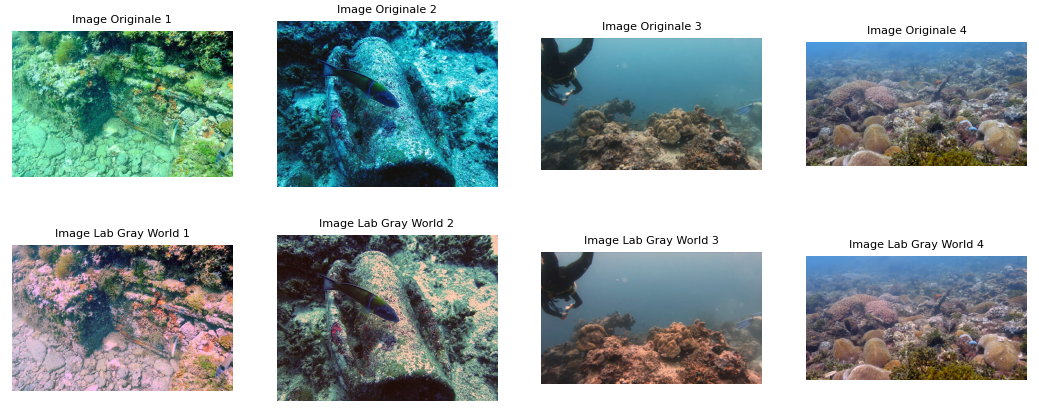
\includegraphics[width=18cm]{image006.png}
\end{center}
\label{figure3.1}
\caption{Résultats de la correction $l\alpha\beta$ (avec l'hypothèse du monde gris) sur des images sous-marines}
\end{figure}  

\begin{figure}[h!]
\begin{center}
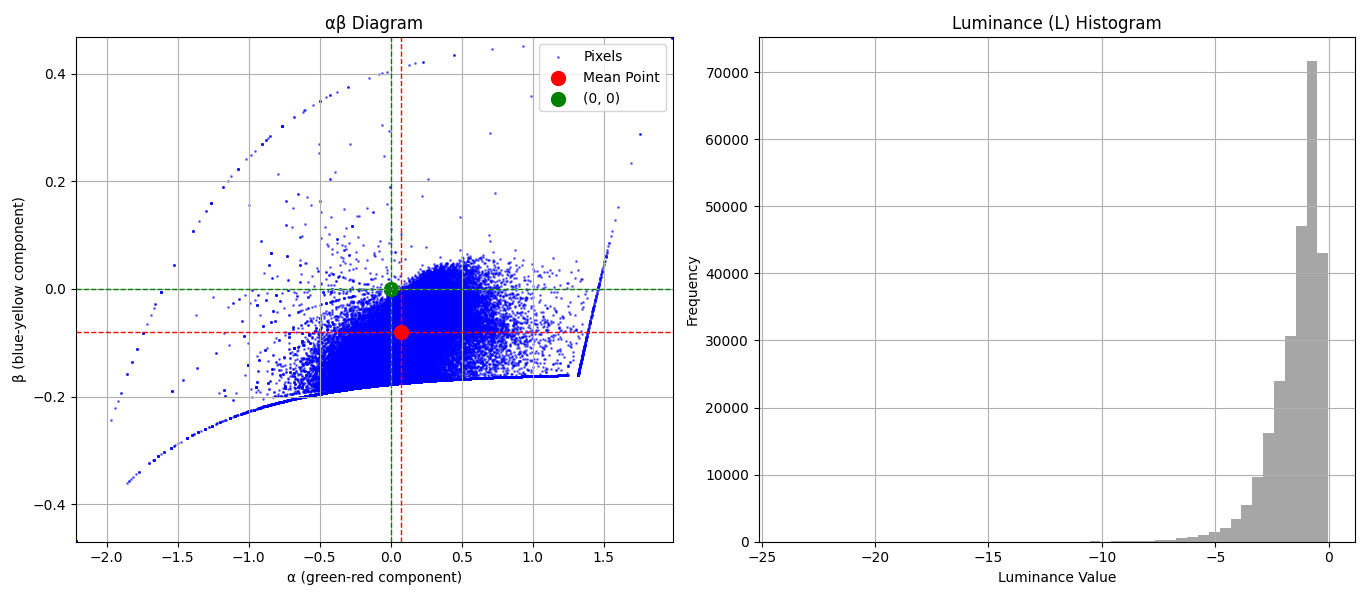
\includegraphics[width=15cm]{image007.png}
\end{center}
\label{figure3.2}
\caption{Diagramme $\alpha\beta$ et Histogramme de la Luminance avant la correction}
\end{figure} 

\begin{figure}[h!]
\begin{center}
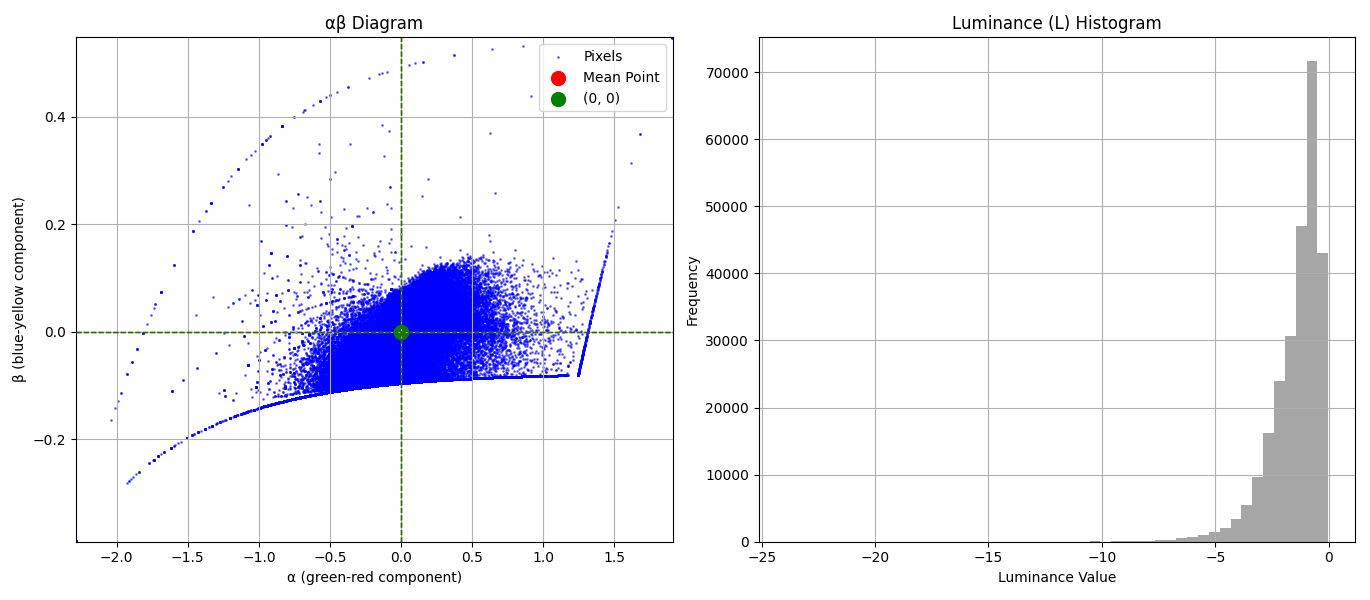
\includegraphics[width=15cm]{image008.png}
\end{center}
\label{figure3.3}
\caption{Diagramme $\alpha\beta$ et Histogramme de la Luminance après la correction}
\end{figure} 

\par Comme on peut l'observer sur la \hyperref[figure3.1]{\textsc{Figure} 3.1} ( le reste des images traitées sont dans le fichier \colorbox{gray!15}{\texttt{\textbf{Images\_Lab\_GW}}}), la correction des couleurs dans l'espace \( l\alpha\beta \) est nettement meilleure que dans l'espace RGB. Cela s'explique par le fait que dans \( l\alpha\beta \), la luminance (\( l \)) est séparée des composantes chromatiques (\( \alpha \) et \( \beta \)). Cette séparation permet d'effectuer des ajustements spécifiques sur les canaux sans altérer la luminosité globale de l'image.

\subsubsection{Hypothèse des White Patches}  
\par Cette méthode ajuste les canaux \( \alpha \) et \( \beta \) en fonction des pixels les plus lumineux (les "patchs blancs"). On identifie les \( p\% \) des pixels les plus lumineux, puis on calcule la moyenne des canaux \( \alpha \) et \( \beta \) pour ces pixels lumineux :
   \[
   \alpha^*(x) = \alpha(x) - \bar{\alpha}_{\text{bright}} \quad\quad\quad \beta^*(x) = \beta(x) - \bar{\beta}_{\text{bright}}
   \]
   où \( \bar{\alpha}_{\text{bright}} \) et \( \bar{\beta}_{\text{bright}} \) sont les moyennes des canaux \( \alpha \) et \( \beta \) pour les pixels lumineux, identifiés en fonction de leur luminance.
\vspace{2mm}   
\par La même observation s'applique qu'à la section \ref{WP} : si l'image d'origine contient des pixels naturellement blancs, elle ne satisfait pas l'hypothèse des patchs blancs, rendant la correction inefficace. En revanche, lorsque l'hypothèse est vérifiée, les résultats obtenus sont comparables à ceux de l'hypothèse du monde gris ( le images traitées sont dans les fichiers \colorbox{gray!15}{\texttt{\textbf{Images\_Lab\_WP\_2p}}} et \colorbox{gray!15}{\texttt{\textbf{Images\_Lab\_WP\_20p}}}).

\subsubsection{Égalisation d'Histogramme sur le Canal \( l \)}

\par Pour améliorer le contraste des images corrigées, une égalisation d'histogramme a été appliquée au canal \( l \) des images traitées selon l'hypothèse du monde gris. Cette opération vise à redistribuer les valeurs de luminance de manière à mieux occuper la plage dynamique disponible.
\vspace{2mm}
\par Soit \( l : \Omega \to [0, 1] \), où \( \Omega \) est le domaine de l'image et les intensités du canal $l$ sont normalisées dans l'intervalle \([0, 1]\). L'égalisation d'histogramme est effectuée via le calcul de l'histogramme cumulé \( F \), défini comme :
\[
F(t) = \frac{1}{N} \; \# \{x \in \Omega : I(x) \leq t \}, \quad\quad t \in [0, 1],
\]
où \( N \) est le nombre total de pixels dans l'image. L'image égalisée est obtenue en appliquant \( F \) sur \( I(x) \), ce qui donne :
\[
I'(x) = F(I(x)).
\]

Lorsque \( F \) est inversible, l'image résultante \( I'(x) \) possède des intensités uniformément réparties, car :
\[
P(F(I) \leq t) = F(F^{-1}(t)) = t.
\]
En pratique, \( F \) n'est pas strictement inversible en raison de la quantification des intensités, mais l'image corrigée présente un histogramme approximativement uniforme. Cette méthode a permis d'améliorer la qualité visuelle des images corrigées comme le montre la \hyperref[figure3.4]{\textsc{Figure} 3.4} ( le reste des images traitées sont dans le fichier \colorbox{gray!15}{\texttt{\textbf{Images\_Lab\_GW\_+\_Eqalization}}}), mais cela fait ressortir plus les composantes rouges des images.

\begin{figure}[h!]
\begin{center}
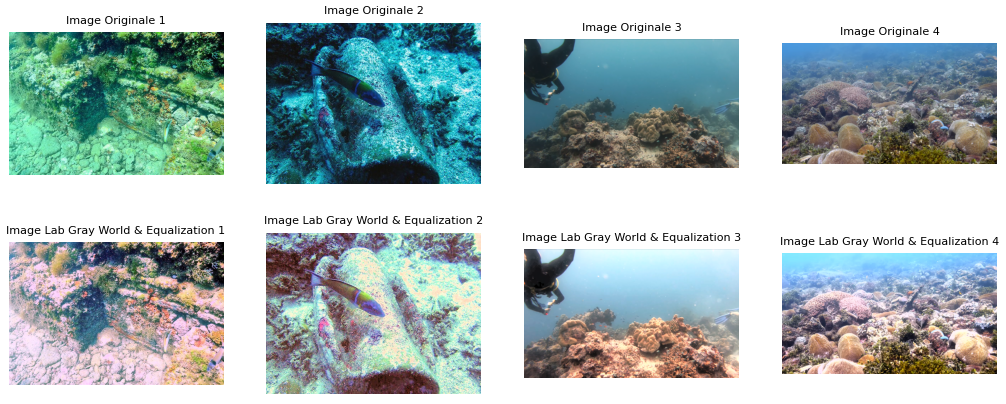
\includegraphics[width=18cm]{image009.png}
\end{center}
\label{figure3.4}
\caption{Résultats de l'égalisation d'histogramme sur le canal $l$ des images de la \hyperref[figure3.1]{\textsc{Figure} 3.1}}
\end{figure} 

\section{Méthode ACE : Égalisation Automatique des Couleurs}
\par Une autre technique qui pourrait nous être utile pour la correction des images sous-marines est l'Automatic Color Equalization (ACE), une méthode conçue pour améliorer à la fois les couleurs globales et locales dans les images. Inspirée par les processus visuels humains, ACE combine deux fonctions essentielles : \textbf{la constance des couleurs}, qui assure une perception cohérente des teintes malgré les variations d'éclairage, et \textbf{l'égalisation de la luminosité}, qui ajuste dynamiquement les contrastes de l'image.
\vspace{2mm}
\par ACE fonctionne en calculant une nouvelle valeur pour chaque pixel en tenant compte des contributions des autres pixels, pondérées par leur distance spatiale et leur différence chromatique. En s'appuyant sur des approches traditionnelles de correction globale telles que \textbf{Gray World} et \textbf{White Patch}, ACE élimine efficacement les dominantes de couleur tout en maintenant un contraste équilibré, tant sur le plan global que local.

\subsection{Modèle et Formulation Mathématique}

\par L'algorithme ACE repose sur une formulation mathématique qui calcule une nouvelle valeur pour chaque pixel d'une image en tenant compte de la distribution spatiale et chromatique de tous les autres pixels. Pour chaque pixel \( x \), la valeur corrigée \( R(x) \) est donnée par :

\begin{equation}
R(x) = \displaystyle\sum_{y \in \Omega \textbackslash x}\dfrac{ s_\alpha(I(x) - I(y))}{d(x-y)}, \quad\quad x\in \Omega
\label{R(x)1}
\end{equation}

où :
\begin{itemize}
    \item[$\bullet$] \( I(x) \) représente l'intensité du pixel \( x \), avec $\quad I\;:\; \Omega \longleftrightarrow [0,1]$.
    \item[$\bullet$] \( s_\alpha \;:\; [-1,1] \longrightarrow \mathbb{R}\) est une fonction de pente (slope function) qui amplifie ou comprime les différences locales selon le paramètre \(\alpha \geq 1\).

\begin{figure}[h]
\begin{center}
\begin{tikzpicture}[scale=1]
    % Axes
    \draw[->] (-3, 0) -- (3, 0) node[right] {\(\Delta I\)};
    \draw[->] (0, -2) -- (0, 2) node[above] {\(s_\alpha(\Delta I)\)};
    
    % Lignes grilles
    \draw[gray, dashed] (-3, 1.5) -- (3, 1.5);
    \draw[gray, dashed] (-3, -1.5) -- (3, -1.5);
    \draw[gray, dashed] (-1, -2) -- (-1, 2);
    \draw[gray, dashed] (1, -2) -- (1, 2);
        
    % Labels
    \node[below left] at (-1, 0) {$-\frac{1}{\alpha}$};
    \node[below right] at (1, 0) {$\frac{1}{\alpha}$};
    \node[below] at (-3, 0) {-1};
    \node[below] at (3, 0) {1};
    
    %Fonction
    \draw[red, very thick] (-3, -1.5) -- (-1, -1.5);
    \draw[red, very thick] (3, 1.5) -- (1, 1.5);
    \draw[red, very thick] (-1, -1.5) -- (1, 1.5);


\end{tikzpicture}
\end{center}
\label{figure4.1}
\caption{Fonction pente $s_\alpha$}
\end{figure} 

\item[$\bullet$] \( d(x, y) \) est une fonction de distance spatiale, typiquement proportionnelle à la distance euclidienne entre \( x \) et \( y \).
\end{itemize}

\par La pondération spatiale permet de moduler l'influence des pixels voisins en fonction de leur distance et de leur intensité relative. Cette combinaison garantit une correction équilibrée entre les ajustements globaux et locaux.
\par Après avoir calculé \( R(x) \), les valeurs sont étirées pour occuper la plage dynamique complète de l'image, généralement entre 0 et 1, avec :

\begin{equation}
L(x) = \frac{R(x) - \min R}{\max R - \min R}
\end{equation}

\par L'algorithme ACE, dans sa forme brute, présente une complexité élevée de \( O(N^4) \), ce qui le rend impraticable pour des images de grande taille. Même pour des images relativement petites, le temps de calcul devient trop long lorsque cette méthode est utilisée en force brute. Il est donc nécessaire de trouver une autre façon d'implémenter cet algorithme afin de le rendre plus efficace.

\subsection{Fonction Pente Polynomiale}
\par Pour résoudre ce problème, la fonction de pente \( s_\alpha \) est approximée par un polynôme, ce qui simplifie les calculs tout en conservant une précision suffisante. Cette approximation réduit la complexité de l'algorithme à \( O(N^2 \log N) \) en utilisant la transformée discrète du cosinus (DCT) pour les convolutions.


\subsubsection{Gestion des Bords de l'Image}
\par Lors des convolutions sur une image, la gestion des bords est un défi. L'extension symétrique à demi-échantillon consiste à répliquer les pixels de bord de manière symétrique en miroir à l'extérieur de l'image pour éviter les artefacts causés par une simple périodisation on un padding.
\par Donc si l'image est de taille $N\times M$ le nouveau domaine \( \mathbb{T}^2 \) qui fait référence à l'ensemble des positions de pixels dans l'image utilisées pour calculer \( R(x) \), est un tore $(2N\!\times\! 2M)$-périodique. L'équation \eqref{R(x)1} devient :

\begin{equation}
R(x) = \sum_{y \in  \mathbb{T}^2} \omega(x - y)s_\alpha(I(x) - I(y)), \quad x \in \mathbb{T}^2
\end{equation}
où $\,\omega : \mathbb{T}^2 \longrightarrow \mathbb{R}_{+}\,$ est une pondération définie par :
$$
\omega(x - y) =
\begin{cases}
0 & \text{si } x = y \\
\dfrac{1}{d(x - y)} & \text{si } x \neq y
\end{cases}
$$
\subsubsection{Approximation Polynomiale}

La fonction de pente $s_\alpha$ est approximée par un polynôme impair, ce qui simplifie les calculs tout en maintenant une précision suffisante. Cette approximation minimise l'erreur maximale sur l'intervalle \([-1, 1]\) en optimisant les coefficients \( c_m \) du polynôme.
$$
\min_{c} \max_{t \in [-1, 1]} \left| s_\alpha(t) - \sum_{m=1}^{D} c_m t^m \right|
$$
Les coefficients optimaux du polynôme pour différentes valeurs de \( \alpha \) peuvent être obtenus via des méthodes d'optimisation telles que l'algorithme de Remez.

\subsubsection{Calcul avec les Convolutions}
\par Cette approximation polynomiale permet de décomposer \( R(x) \) en une somme de convolutions :

\begin{equation}
R(x) = \sum_{n=0}^{D} a_n\left(I(x)\right) \left( \omega * I^n \right)(x)
\end{equation}

où :
\begin{itemize}
\item[$\bullet$] \( \omega * I^n \) est une convolution cyclique sur \( \mathbb{T}^2 \).
\item[$\bullet$]  \( a_n\left(t\right) \) un polynôme défini par :
$$
\sum_{m=n}^{D} c_m \binom{m}{n} (-1)^{m-n+1} t^{m-n}
$$
\end{itemize}

 Les convolutions peuvent être efficacement calculées avec les transformations DCT en \( O(N^2 \log N) \) opérations.et pour une image couleur RGB, \( 3M \) convolutions doivent être calculées. La sommation sur \( n \) peut être parallélisée, puisque l'évaluation de \( a_n(x) \left( \omega * I_n \right)(x) \) est indépendante pour chaque \( n \), mais ça n'a pas été utilisé ici.

\subsection{Implémentation pour la Correction des Images Sous-marines}
\subsubsection{Test de l'ACE sur des Images Synthétiques}

\par La méthode ACE a été initialement implémentée à travers le programme \colorbox{gray!15}{\texttt{\textbf{Undermarine\_test2.py}}} qui utilise la fonction \colorbox{gray!15}{\texttt{\textbf{ace\_enhance\_image\_poly}}} pour des images synthétiques afin d'évaluer son efficacité dans des conditions idéales et d'observer les caractéristiques du filtrage. Certaines de ces propriétés dépendent des paramètres de l'algorithme, tandis que d'autres sont influencées par le contenu de l'image. À moins d'indication contraire, les résultats présentés dans ici utilisent :
\begin{itemize}
	\item[$\bullet$] $\,\alpha = 7$.
    \item[$\bullet$]  Un polynôme $c$ de degré $D = 11$. 
    \item[$\bullet$]  Une distance euclidienne.
\end{itemize}

\begin{figure}[h]
\begin{center}
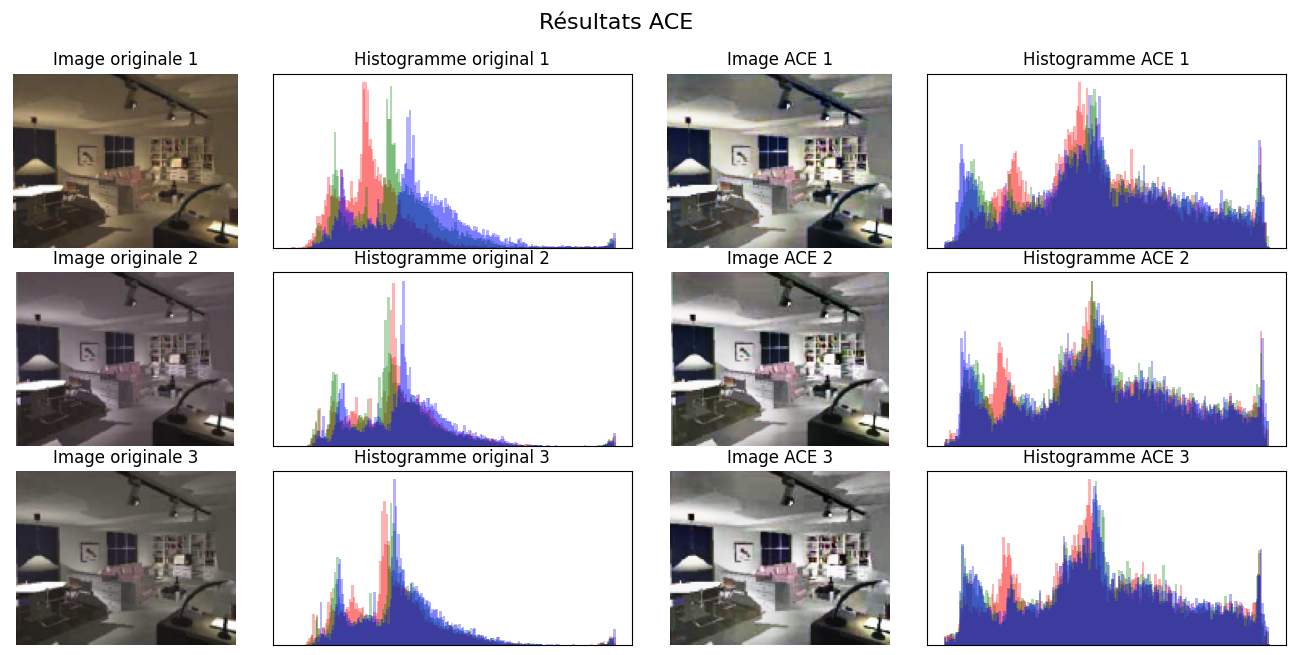
\includegraphics[width=18cm]{image001.png}
\end{center}
\label{figure4.2}
\caption{Résultats de l'ACE sur des images synthétiques}
\end{figure} 

\par On remarque L'ACE ajuste automatiquement la luminosité et la dynamique de l'image en fonction de sa luminosité d'origine, contrairement à d'autres algorithmes qui augmentent systématiquement la luminosité. Par exemple, il augmente la luminosité d'une image sous-exposée et la réduit pour une image surexposée. L'impact de l'algorithme sur la dynamique est visible dans les histogrammes avant et après filtrage ACE. Quantitativement, les effets sur la luminosité et la dynamique sont mesurés par :
\begin{itemize}
\item[$\bullet$]\textbf{Lissage de l'histogramme :} distance $L^1$ entre l'histogramme de l'image et un histogramme plat.
\item[$\bullet$]\textbf{Pourcentage de dynamique utilisée :} proportion des valeurs dans l'étendue dynamique disponible.
\item[$\bullet$]\textbf{Pourcentage de noir/blanc inutilisés :} fraction de valeurs inutilisées aux extrémités de l'étendue dynamique.
\end{itemize}
\vspace{2mm}

\subsubsection{Correction des Images Sous-marines avec l'ACE}

\par Nous appliquons maintenant la méthode aux images sous-marines utilisées précédemment. Cependant, nous rencontrons les mêmes problèmes observés plus tôt : pour les images dont la composition s'éloigne de l'hypothèse du monde gris, en particulier dans les zones maritimes avec de grandes étendues d'eau, l'algorithme tend à accentuer la teinte rouge, comme on le voit dans l'exemple du corail. Bien que les résultats obtenus avec l'espace $l\alpha\beta$ soient similaires à ceux des précédents essais, cette méthode est globalement plus performante. En effet, l'amélioration du contraste est meilleure, comme on peut le constater dans la \hyperref[figure4.3]{\textsc{Figure} 4.3} ( le reste des images traitées sont dans le fichier \colorbox{gray!15}{\texttt{\textbf{Images\_ACE\_(alpha7-deg11-dist)}}}).  

\begin{figure}[h!]
\begin{center}
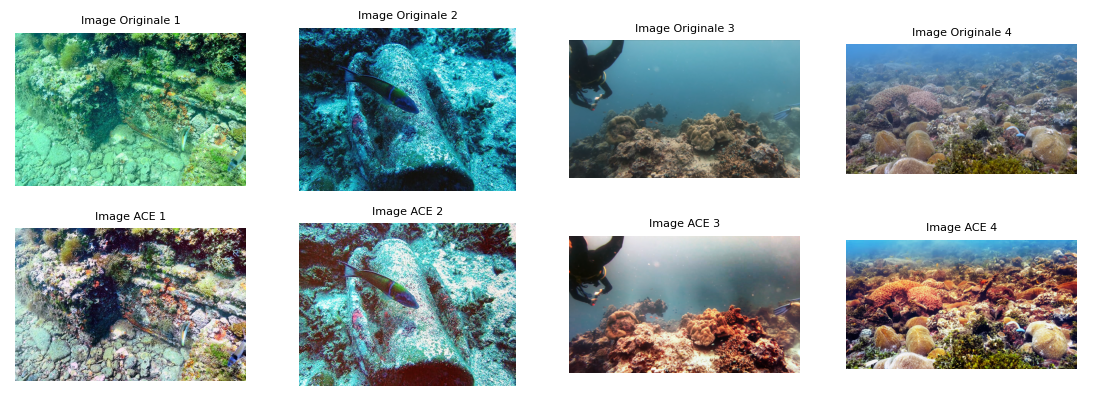
\includegraphics[width=18cm]{image002.png}
\end{center}
\label{figure4.3}
\caption{Résultats de l'ACE sur les images sous-marines}
\end{figure} 

\subsubsection{Application de l'ACE sur le Canal \( l \)}

\par Une autre approche implémentée consiste à appliquer l'ACE uniquement sur le canal $\,l\,$ après une transformation dans l'espace colorimétrique $l\alpha\beta$, dans le but d'améliorer le contraste et la luminosité de l'image. Cela est réalisé via la fonction \colorbox{gray!15}{\texttt{\textbf{process\_underwater\_image}}}, avec des ajustements apportés à la fonction \colorbox{gray!15}{\texttt{\textbf{gray\_world\_lab}}}, tout en supposant l'hypothèse du monde gris. Comme illustré dans la \hyperref[figure4.4]{\textsc{Figure} 4.4} ( le reste des images traitées sont dans le fichier \colorbox{gray!15}{\texttt{\textbf{Images\_Lab\_GW\_+\_ACE(L)}}}, cette méthode permet une augmentation notable de la luminosité. Cependant, le contraste global en ressort réduit par rapport à l'application de l'ACE sur les trois canaux RGB. En outre, une différence importante réside dans la gestion des couleurs : contrairement à l'égalisation d'histogramme, qui équilibre les teintes de manière uniforme, l'ACE met fortement en avant la composante rouge de l'image. 

\begin{figure}[h!]
\begin{center}
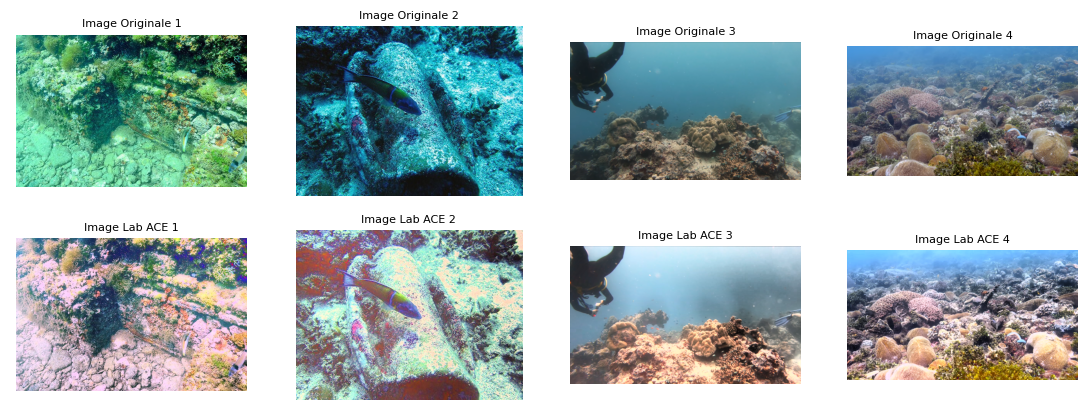
\includegraphics[width=18cm]{image003.png}
\end{center}
\label{figure4.4}
\caption{Résultats de l'ACE sur le canal $l$ des images de la \hyperref[figure3.1]{\textsc{Figure} 3.1}}
\end{figure} 

\section{Conclusion}
\par Comme nous avons pu le constater, la diversité des méthodes étudiées et expérimentées offre un large éventail de possibilités pour l'amélioration des images sous-marines. Chaque méthode possède des avantages. Toutefois, ces techniques présentent également des limites, notamment en termes de complexité computationnelle et d'adaptabilité à des conditions variées.

\vspace{3mm}

\par Lorsque l’on s’oriente vers des applications en temps réel, comme l’analyse de vidéos pour des robots sous-marins ou des systèmes de surveillance, la rapidité des algorithmes devient un critère essentiel. Les méthodes classiques, bien qu'efficaces dans des contextes spécifiques, peinent à répondre à cette exigence en raison du temps de traitement nécessaire. De ce fait, une approche moderne, basée sur l’exploitation de modèles d’apprentissage profond préalablement entraînés, s’impose comme une solution prometteuse. Ces modèles permettent de combiner \textbf{efficacité}, \textbf{rapidité} et \textbf{qualité}.


\newpage
\listoffigures
\addcontentsline{toc}{section}{Table des figures}
\newpage
\begin{thebibliography}{99}
\begin{doublespace}
\addcontentsline{toc}{section}{R\'ef\'erences}
\bibitem{1} R. Schettini and S. Corchs, "Underwater Image Processing: State of the Art of Restoration and Image Enhancement Methods," \textit{EURASIP Journal on Advances in Signal Processing}, vol. 2010, Article ID 746052, 2010, doi: 10.1155/2010/746052.
\bibitem{2} G. Bianco, M. Muzzupappa, F. Bruno, R. Garcia, and L. Neumann, "A New Color Correction Method for Underwater Imaging," \textit{The International Archives of the Photogrammetry, Remote Sensing and Spatial Information Sciences}, vol. XL-5/W5, pp. 16–17, 2015, Underwater 3D Recording and Modeling, 16–17 April 2015, Piano di Sorrento, Italy.
\bibitem{3} E. Reinhard, M. Ashikhmin, B. Gooch, and P. Shirley, "Color Transfer between Images," \textit{Applied Perception}, vol. 34, September/October 2001.
\bibitem{4} A. Rizzi, C. Gatta, and D. Marini, "A New Algorithm for Unsupervised Global and Local Color Correction," \textit{Department of Information Technology, University of Milano}, 2001.
\bibitem{5} P. Getreuer, "Automatic Color Enhancement (ACE) and its Fast Implementation," \textit{Image Processing On Line}, 2012, doi: 10.5201/ipol.2012.g-ace.
\bibitem{6} J. Han, M. Shoeiby, T. Malthus, E. Botha, J. Anstee, S. Anwar, R. Wei, M. A. Armin, H. Li, and L. Petersson, ``Underwater Image Restoration via Contrastive Learning and a Real-World Dataset,'' \textit{Remote Sensing}, vol. 14, no. 17, p. 4297, 2022. \url{https://doi.org/10.3390/rs14174297}.

  
\end{doublespace}   
\end{thebibliography}

\end{document}